\subsection{SKAによる突発天体探査}\label{transients.s2.fender}
第~\ref{transients.s1}節および次節以降で述べるように、宇宙における突発現象は極めて高エネルギーな現象が元になっていると考えられ、その観測的研究によって新たな物理が開拓される可能性を秘めている。
ただし、突発現象は宇宙のいつどこで起こるかということが予測することができないため、探査のみをやみくもに続けることはリスクが高い。
しかしこのことは裏を返せば、突発天体の探査は他の目的の観測と並行して実施できるということである。
また突発現象は、初期の増光段階と時間経過後の減光段階で、電波放射の物理過程が異なることもあり、現象が発生した直後から継続して追観測することが重要である。
そのような特徴や課題をもつ突発現象の観測的研究では、以下の二つの機能をSKAに実装することが重要な鍵となる:
\begin{itemize}
	\item[(1)] 他の目的による観測と共存・並行して運用できる、突発天体の探査観測システム、
	\item[(2)] 突発天体が発見された際に、それを即時的・自動的に追観測するシステム。
\end{itemize}
本節ではこの二つの機能について紹介する。

%%
\subsubsection{SKAへの要求 (1): 他の観測と共存する突発天体探査システム}
%%
探査によって突発現象を発見できるかどうかは確率によって評価できるが、多かれ少なかれ運に左右される。
しかし一方で、探査は他の目的の観測と並行して実施することができ、多大な観測時間を費やすことができるという大きなメリットがある。
観測時間が多ければ多いほど突発現象を発見できる確率は上がるため、その探査システムを他の観測と共存できるように構築することで、効率的に探査ができるようになり大きな科学成果を期待できる。

そのようなシステムとして、例えば図~\ref{fig:transients.fender.commensal}に示すようなシステムをアフリカのMeerKATに実装することが提案されている (Armstrong et al., in prep)。
この共存システムは、観測データの処理経路を分岐させ、一方を本来の観測のために使用し、もう一方を突発天体のリアルタイム探査に使用するというものである。
図~\ref{fig:transients.fender.commensal}は観測データの流れと処理過程を示しており、図左上の相関器 (correlator) から処理が始まる。
通常の観測では、相関器から出力される電波干渉計のデータに対して図右方向に向かってさまざまな解析処理を施し、最終的に輝度分布画像を得る。
その観測には通常数時間以上を費やし、その長時間の観測データを後日取りまとめる場合が多い。
一方で突発天体は、その変動のタイムスケールが観測時間よりも短い可能性があり、またその追観測には即時性を要する。
そのため突発天体探査は通常観測だけでは不十分であり、リアルタイムにデータ処理を行う必要がある。
そこで通常観測と共存する形で処理経路を分岐させ、即座に簡易的な画像データを得て天体の光度変動を検出する。
それを行うのが図~\ref{fig:transients.fender.commensal}の左半分に示されるシステムである。
もし突発天体が検出されれば、自動的にその情報を VOEventNet と呼ばれる突発天体の発見速報ネットワークに通報する。
その通報によって、世界中の他の観測局がその突発天体を追観測することができれば、その起源や放射機構について詳しい情報が得られることだろう。
\begin{figure}
	\centering
	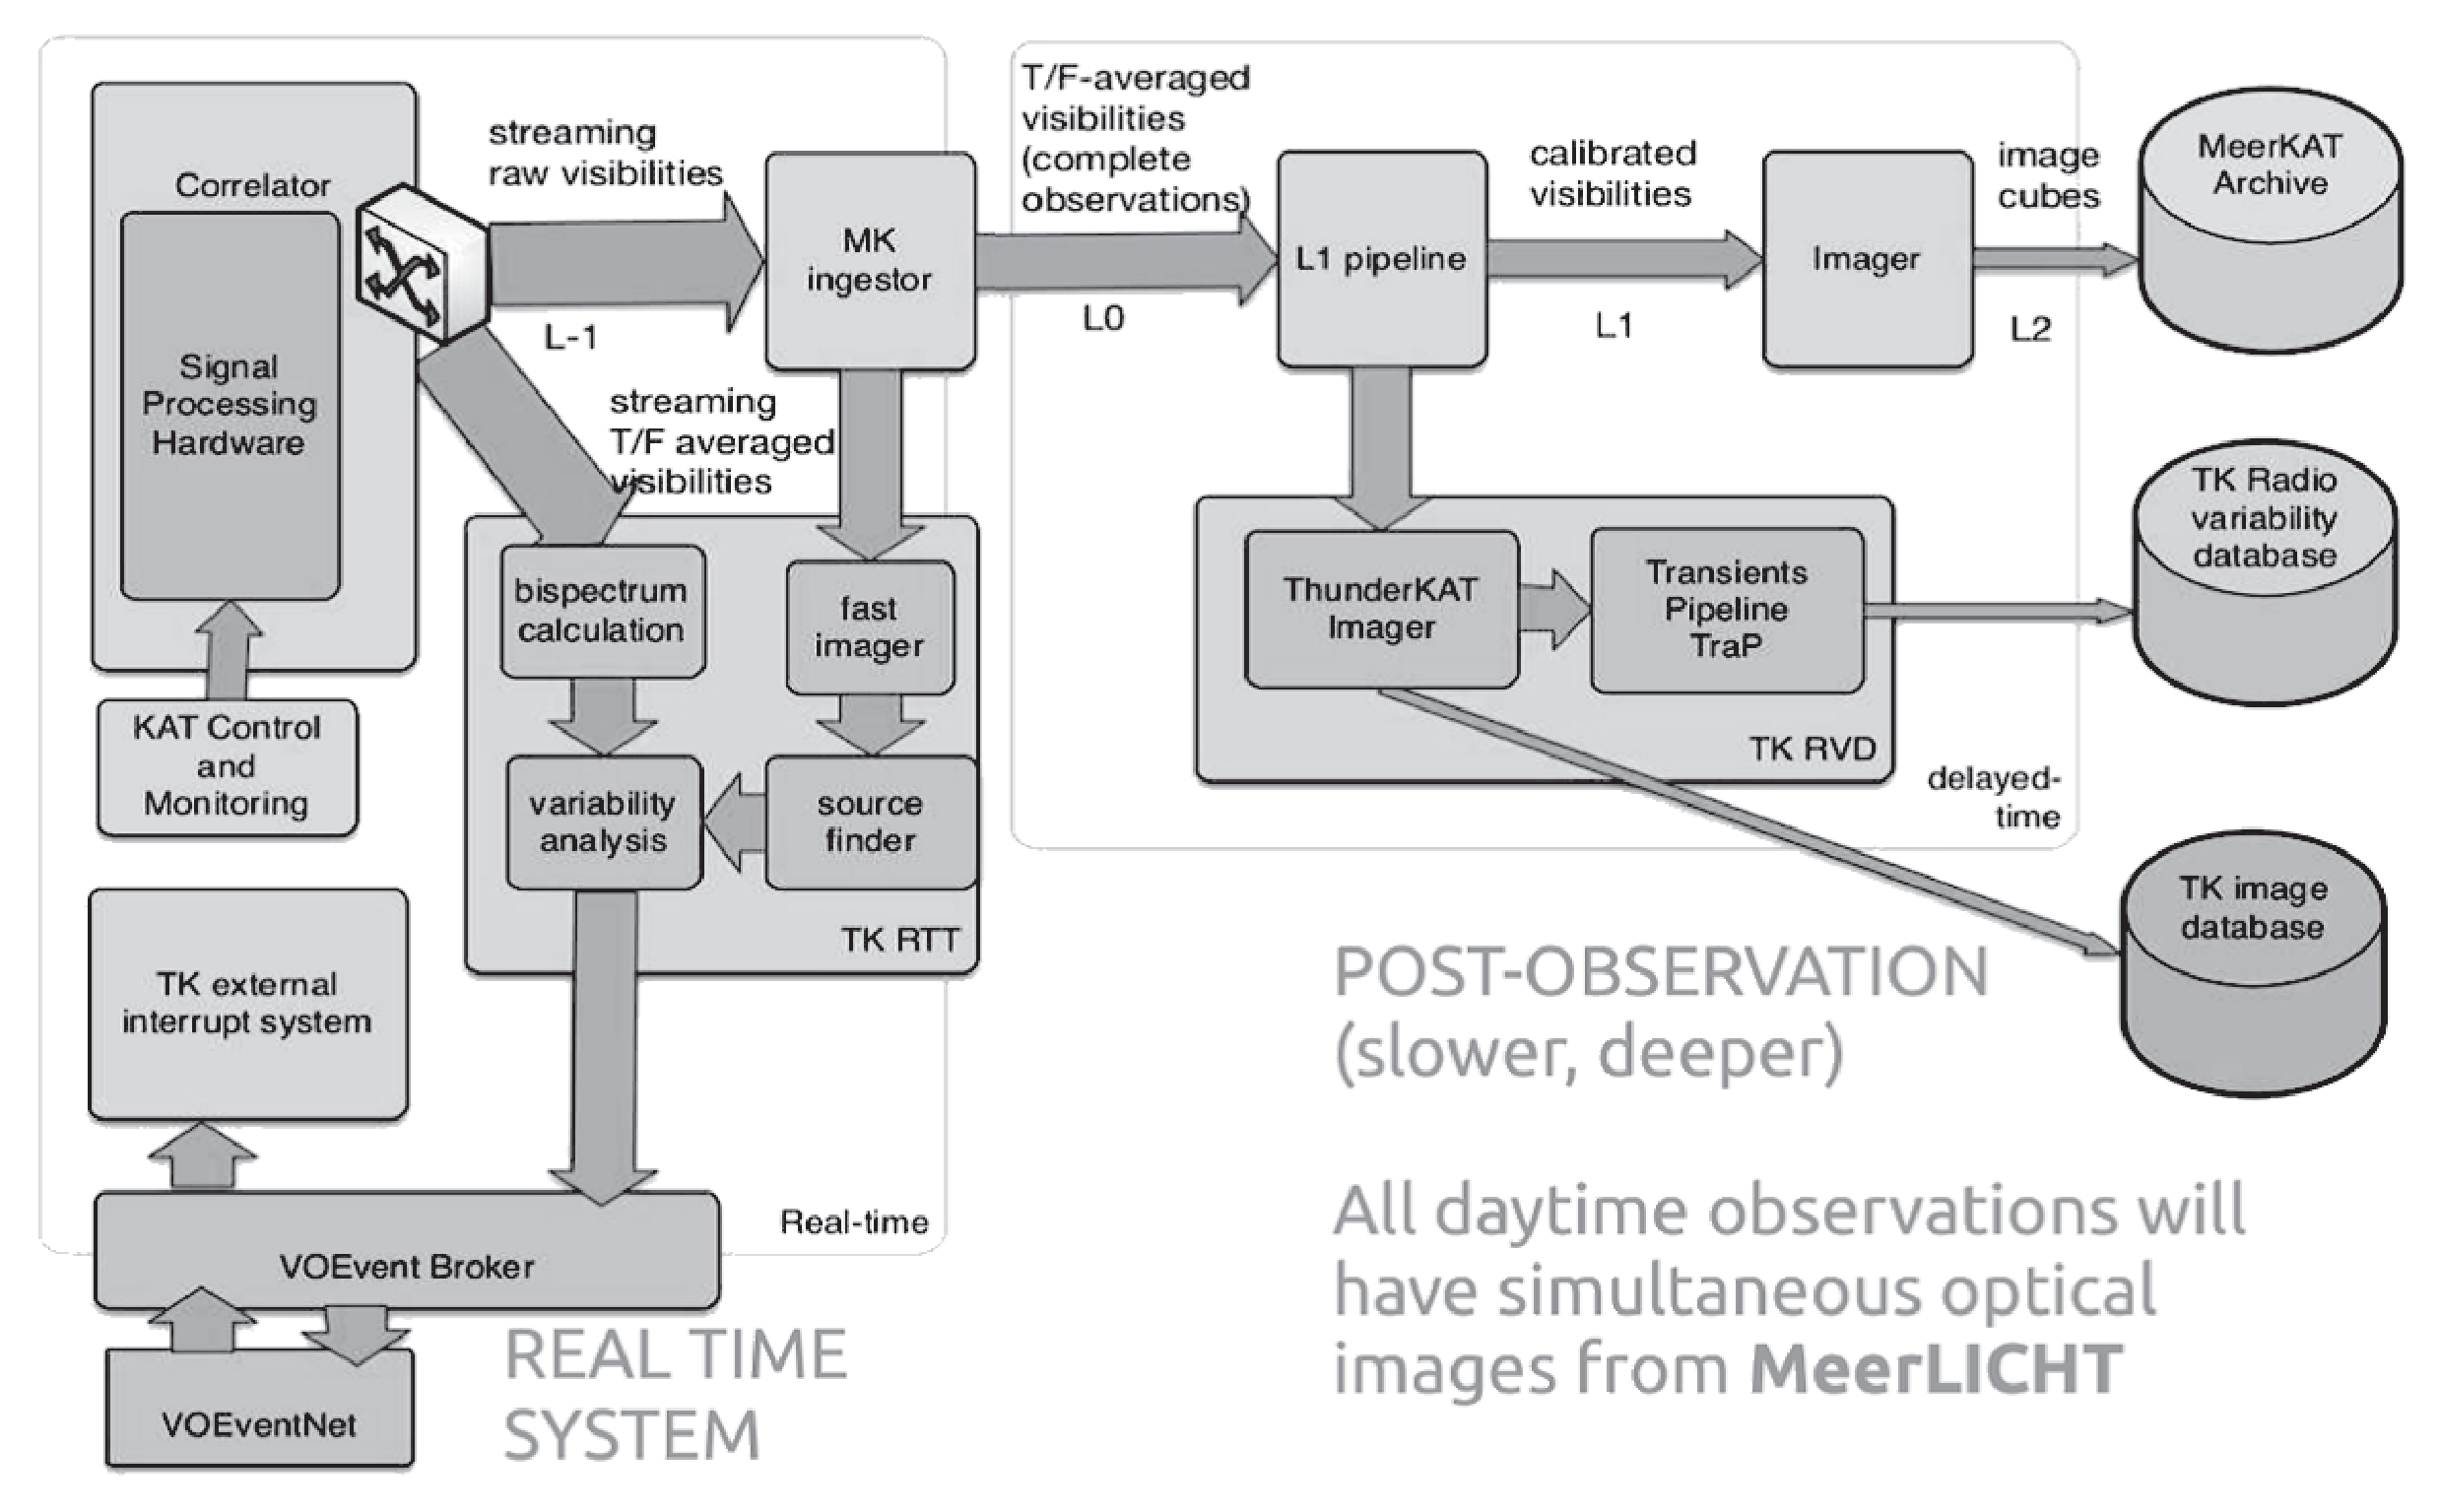
\includegraphics[width=12cm]{transients/transients.s2.fender.commensal.eps}
	\caption{他の観測と共存した突発天体探査システム。}
	\label{fig:transients.fender.commensal}
\end{figure}%

%%
\subsubsection{SKAへの要求 (2): 突発天体発見時の自動的な追観測システム}
%%
突発天体の観測的研究に重要なもう一方のシステムは、他の観測局によって発見された突発天体、あるいはSKA自身によって発見した突発天体を、自動的に追観測するというものである。
このようなシステムは既にイギリスのArcminute Microkelvin Imager Large Array (AMI LA) に実装されており、ガンマ線観測衛星Swiftで発見されたガンマ線バーストを約8時間後に追観測することに成功している \citep{2013MNRAS.428.3114S,2014MNRAS.440.2059A}。
この結果得られた電波帯域での光度曲線から、ガンマ線バーストのリバースショック (星間物質から噴出物の方向に伝わる衝撃波) による電波放射が、世界で初めて確認された。
同様にSwiftの速報によって、地球近傍の連星系 DG~CVn からのガンマ線フレアを6分以内に追観測した結果、電波帯域でも大きいフレアが確認され、広い周波数帯域でのコインシデンスが得られている。
しかし数日後には元の明るさに戻ってしまい、そのようなタイムスケールの短い突発現象を詳細に観測するためには、世界規模で即時的な追観測を行うことが重要である \citep{2015MNRAS.446L..66F}。
SKAにおいても同様のシステムを実装すれば、突発天体の研究にブレイクスルーを起こすことができるだろう。

%%
\subsubsection{まとめ}
%%
突発天体の観測的研究には、SKAに前述の二つのシステムを実装することが重要である。
SKAは広い視野と高い感度を兼ね備えており、さらにそのシステムが実装されれば、電波帯域での変動天体や突発天体を数多く発見することができるだろう。
その発見は、究極の宇宙物理を議論できる場所に、人類を導いてくれるはずである。
突発現象というのは宇宙の、とりわけ深宇宙の灯台であり、その観測によって新しい物理を開拓できるに違いない。

